\documentclass[journal]{IEEEtran}
\usepackage[a5paper, margin=10mm, onecolumn]{geometry}
\usepackage{lmodern}
\usepackage{tfrupee}
\setlength{\headheight}{1cm}
\setlength{\headsep}{0mm}

\usepackage{gvv-book}
\usepackage{gvv}
\usepackage{cite}
\usepackage{amsmath,amssymb,amsfonts,amsthm}
\usepackage{algorithmic}
\usepackage{graphicx}
\usepackage{textcomp}
\usepackage{xcolor}
\usepackage{txfonts}
\usepackage{listings}
\usepackage{enumitem}
\usepackage{mathtools}
\usepackage{gensymb}
\usepackage{comment}
\usepackage[breaklinks=true]{hyperref}
\usepackage{tkz-euclide}
\usepackage{listings}
\def\inputGnumericTable{}
\usepackage[latin1]{inputenc}
\usepackage{color}
\usepackage{array}
\usepackage{longtable}
\usepackage{calc}
\usepackage{multirow}
\usepackage{hhline}
\usepackage{ifthen}
\usepackage{lscape}
\usepackage{xparse}
\bibliographystyle{IEEEtran}
\title{12.56}
\author{EE25BTECH11043 - Nishid Khandagre} 
\begin{document}
\maketitle

\renewcommand{\thefigure}{\theenumi}
\renewcommand{\thetable}{\theenumi}

\numberwithin{equation}{enumi}
\numberwithin{figure}{enumi}
\textbf{Question}:\
The area enclosed between the curves $y^2 = 4x$ and $x^2 = 4y$ is 

\textbf{Solution}:\\
The equation of a parabola in Matrix form is
\begin{align}
\vec{x}^\top\vec{V}\vec{x} + 2\vec{u}^\top\vec{x} + f = 0
\end{align}
For $y^2 = 4x$:
\begin{align}
    \vec{V_1}=\begin{pmatrix}
        0 & 0\\
        0 & 1
    \end{pmatrix}\\
    \vec{u_1}=-2\vec{e_1}=\myvec{-2\\0}\\
    f_1=0
\end{align}
For $x^2 = 4y$:
\begin{align}
    \vec{V_2}=\begin{pmatrix}
        1 & 0\\
        0 & 0
    \end{pmatrix}\\
    \vec{u_2}=-2\vec{e_2}=\myvec{0\\-2}\\
    f_2=0
\end{align}
The intersection of two conics with parameters $\vec{V_i}$, $\vec{u_i}$, $f_i$, $i=1,2$ is defined as 
\begin{align}
\vec{X}^{T}\,(\vec{V}_{1} + \mu \vec{V}_{2})\vec{X} + 2(\vec{u_1} + \mu \vec{u_2})^{T}\vec{X} \;+\; (f_{1} + \mu f_{2}) \;=\; 0 \label{eq:tem}
\end{align}
\begin{align}
\implies \left|
\begin{array}{cc}
\mathbf{V}_1 + \mu \mathbf{V}_2 & \mathbf{u}_1 + \mu \mathbf{u}_2 \\[6pt]
(\mathbf{u}_1 + \mu \mathbf{u}_2)^{\mathrm{T}} & f_1 + \mu f_2
\end{array}
\right| = 0
\end{align}
\begin{align}
    \implies 
\left|
\begin{array}{ccc}
\mu & 0 & -2 \\[6pt]
0 & 1  & -2\mu \\[6pt]
-2 & -2\mu & 0
\end{array}
\right| = 0 \\
\implies \left|
\begin{array}{ccc}
\mu & 0 & -2 \\[6pt]
0 & 1  & -2\mu \\[6pt]
-2 & -2\mu & 0
\end{array}
\right| &\xleftrightarrow{R_3 \leftrightarrow R_3 + \frac{2}{\mu}\times R_1} \left|
\begin{array}{ccc}
\mu & 0 & -2 \\[6pt]
0 & 1  & -2\mu \\[6pt]
0 & -2\mu & -\frac{4}{\mu}
\end{array}
\right|\\
&\xleftrightarrow{R_3 \leftrightarrow R_3 + 2\mu \times R_2} \left|
\begin{array}{ccc}
\mu & 0 & -2 \\[6pt]
0 & 1  & -2\mu \\[6pt]
0 & 0 & -(\frac{4}{\mu} +4 \mu ^2)
\end{array}
\right| =0\\
\implies -(4 + 4 \mu ^3)=0\\
\implies \mu=-1
\end{align}
Substituting the value of $\mu=-1$ in $\eqref{eq:tem}$ we get points of intersection as 
\begin{align}
    \vec{x_1}=\myvec{0\\0} \\
    \vec{x_2}=\myvec{4\\4}
\end{align}
Area of the desired region is given by
\begin{align}
A &= \int_{0}^{4}\left(2\sqrt{x}-\frac{x^2}{4}\right)dx\\
A &= \left[\frac{4}{3}x^{3/2} - \frac{x^3}{12}\right]_{0}^{4}\\
A &= \left(\frac{4}{3}(4)^{3/2} - \frac{(4)^3}{12}\right) - \left(0 - 0\right)\\
A &= \left(\frac{4}{3}(8) - \frac{64}{12}\right)\\
A &= \left(\frac{32}{3} - \frac{16}{3}\right)\\
A &= \frac{16}{3}
\end{align}
Thus, the area enclosed between the curves is $\frac{16}{3}$.
\begin{figure}[H]
\centering
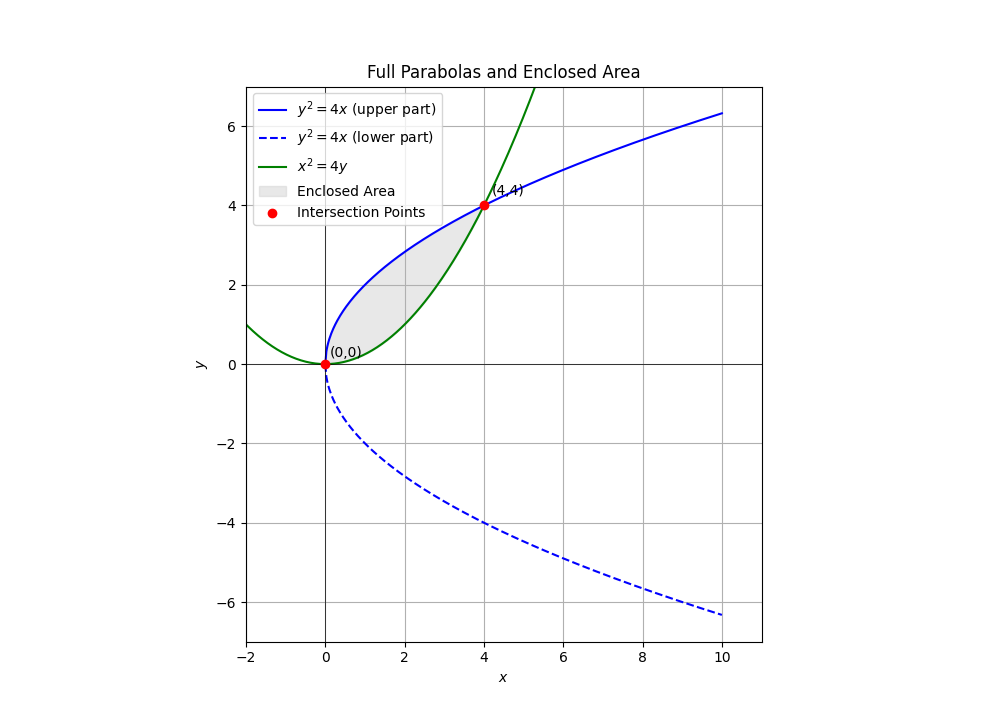
\includegraphics[width=0.8\columnwidth]{figs/fig1.png}
\caption{}
\label{fig:1}
\end{figure}
\end{document}
